%%%%%%%%%%%%%%%%%%%%%%%%%%%%%%%%%%%%%%%%%%%%%%%%%%%%%%%%%%%%%%%%%%%%%%%%%%%%%%%%
%%%                               80 COLONNES                                %%%
%%%%%%%%%%%%%%%%%%%%%%%%%%%%%%%%%%%%%%%%%%%%%%%%%%%%%%%%%%%%%%%%%%%%%%%%%%%%%%%%

\chapter{Plates-formes logicielles~: évaluation, problèmes et améliorations}
\chaptermark{Plates-formes logicielles}
\label{ChPFLogicielles}

Une étape essentielle de nos travaux a consisté à chercher une plate-forme
logicielle (c'est-à-dire un système d'exploitation) spécialisée dans les
réseaux de capteurs sans-fil et présentant les caractéristiques adéquates
pour nos travaux~; ces travaux consistant notamment à implanter et à
évaluer les performances des protocoles réseaux avancés décrits dans
la section \vref{SubsecProtoMACavances} du présent manuscrit.

Suite à l'analyse de l'état de l'art sur les systèmes d'exploitation dédiés
(cf. section \vref{SecOSWSN}), nous avons retenu deux plates-formes
logicielles de travail~: la référence actuelle, Contiki OS (décrit
en section \vref{SubsecContikiOS}), et celle nous semblant la plus
prometteuse du point du vue fonctionnel, RIOT OS (détaillée dans
la section \vref{SubsecRIOTOS}).

\medskip

Cette tâche s'est révélée plus longue et ardue que nous ne l'avions
imaginé \textit{a priori}, les systèmes de référence établis de longue
date ne convenant pas à nos besoins.

%%%%%%%%%%%%%%%%%%%%%%%%%%%%%%%%%%%%%%%%%%%%%%%%%%%%%%%%%%%%%%%%%%%%%%%%%%%%%

\section{Contiki~: développement et limitations}
\label{SecLimContiki}

Notons que nous avons dès le départ écarté TinyOS, pour toutes les raisons
décrites dans la section \vref{SubsecTinyOS} qui lui est consacrée.
Notre premier choix de plate-forme logicielle a donc été logiquement
le système de référence actuel, Contiki OS.

Comme indiqué précédemment dans la section \vref{SubsecContikiOS}, les
qualités proposées par ce système, notamment le support actif des communautés
tant académique qu'industrielle, en faisait un choix de départ logique pour
effectuer nos développements.

En outre, ce système est depuis 2011 fourni avec son propre protocole MAC,
ContikiMAC (décrit en section \vref{ParContikiMAC}), lequel est désormais
le protocole utilisé par défaut par Contiki. Ce protocole est ainsi devenu
le standard de fait dans nombre de publications récentes dans le domaine
des réseaux de capteurs sans-fil.

L'une des premières tâches à laquelle nous nous sommes attelés est ainsi
d'implanter S-CoSenS (décrit dans la section \vref{ParSCoSenS} sur nos
protocoles avancés) afin de pouvoir effectuer une comparaison équitable
entre ce protocole et ContikiMAC. Nous avons préféré commencer par
implanter ce protocole plutôt qu'iQueue-MAC, nettement plus
performant mais aussi plus complexe à implanter.

L'intégration de S-CoSenS dans la pile réseau Contiki devait notamment nous
permettre d'évaluer l'influence de toutes les couches de la pile réseau, et 
l'interaction de celles-ci avec chaque protocole MAC~/ RDC, afin d'obtenir
des résultats les plus fidèles possibles à la réalité du déploiement
d'un réseau de capteurs sans-fil en production.

\bigskip

Malheureusement, durant notre effort d'implantation du protocole S-CoSenS
au sein de la pile réseau (\lang{``netstack''}) de Contiki, nous avons fait
face à de nombreux problèmes nuisant au développement à l'intérieur de ce
système, tant au niveau général que dans le domaine plus spécifique de
la pile réseau \cite{KR-RR-8776-2013}.
Nous allons dans la présente section décrire les problèmes
rencontrés, en tentant~--- quand cela est possible~--- de proposer des
solutions ou tout au moins des moyens de contournement.


\subsection{Documentation minimaliste}
\label{SubsecDocContiki}

Ceci est un problème récurrent avec Contiki~: à l'exception du code source
du système et des exemples d'applications fournis, il n'y a quasiment aucune
documentation. Ceci concerne de façon générale l'ensemble de Contiki,
y compris et notamment sa pile réseau.

On regrettera notamment l'absence totale de documents techniques de référence,
où l'architecture générale du système, les choix de conception et
d'implantation seraient expliqués~; une telle documentation de référence
représente un outil essentiel pour réellement comprendre une plate-forme
logicielle, et ainsi permettre aux développeurs débutants de devenir
rapidement efficaces dans leur travail.

Il y a également très peu de documents d'introduction (<<~tutoriels~>>)~:
le seul document d'initiation officiel est la page \lang{``get started''} du
site Web du projet Contiki. Celle-ci montre comment télécharger et utiliser
la distribution Linux dédiée au test du système, nommée \lang{``Instant
Contiki''}, pour effectuer rapidement des simulations de réseaux de capteurs
sans-fil~--- grâce à l'utilisation du simulateur \nom{Cooja} \cite{Cooja}
fourni par le projet Contiki~--- puis télécharger des programmes d'exemple
sur du matériel (des \lang{motes} de type Zolertia Z1). Aucun document n'est
disponible pour montrer et (plus important encore) expliquer aux
développeurs les nombreuses fonctionnalités de Cooja~; aucun document pour
détailler comment programmer des applications avec Contiki~; aucune
introduction signalant quelles sont les spécificités du développement
embarqué sur des systèmes aussi contraints que les \lang{motes} constituant
les réseaux de capteurs sans-fil (par opposition au développement
<<~classique~>> sur PC). Enfin, l'absence de documentation sur le
fonctionnement interne de Contiki, et sur les méthodes éventuelles
pour adapter le système à ses propres besoins, est particulièrement
regrettable pour qui souhaite mener des travaux concrets de recherche
et de développement avec, et surtout \emph{dans} ce système~--- or,
de telles initiatives d'exploitation <<~avancée~>> sont appelées
à être relativement nombreuses, étant donné le statut d'OS pour WSN
de référence que possède actuellement Contiki.

En résumé, une telle absence de documentation raisonnablement accessible
rend l'approche initiale de Contiki difficile pour les nouveaux développeurs,
et contribue à leur imposer une courbe d'apprentissage relativement élevée.

La principale source de documentation, en matière de développement sous
Contiki, est la \lang{mailing-list}
\texttt{"contiki-developers"}\footnotemark[1].
Toute personne souhaitant développer sur cette plate-forme logicielle
(qu'il s'agisse d'applications ou au niveau du système) ne peut espérer
atteindre un quelconque but sérieux sans souscrire à cette liste, et
demander de l'aide et des renseignements à ses membres. Bien que cette
liste soit une source riche d'informations, soit réactive, et en
général bien disposée à l'égard des nouveaux venus, on peut difficilement
considérer qu'elle remplace de façon satisfaisante le manque de
documentation technique et de tutoriels.

\footnotetext[1]{
Adresse~: \texttt{contiki-developers@lists.sourceforge.net}\\
URL de gestion~:
\texttt{https://lists.sourceforge.net/lists/listinfo/contiki-developers}
}

Ajoutons également que, si de nombreux exemples d'applications conçues
avec le système Contiki sont fournis avec le code source du système,
il n'y a par contre aucun exemple de code destiné à s'insérer dans
le système lui-même (comme par exemple un \lang{plug-in} pour la pile
réseau ou toute autre partie du c{\oe}ur du système). Le développement
au sein du système Contiki, par exemple pour l'adapter à ses besoins
ou y rajouter des fonctionnalités, n'en est ainsi qu'encore plus
difficile à apprendre et à maîtriser.


\subsection{Limitations techniques}
\label{SubsecLimContiki}

De nombreuses limitations du système Contiki ont été dictées par les
contraintes fortes imposées par les appareils constituant les réseaux de
capteurs sans-fil~: ces noeuds sont en effet extrêmement limités quant à
leur puissance de calcul et (surtout) leur espace mémoire disponible.

Nous étudierons dans cette section ces différentes limitations, certaines
étant dues à des problèmes plus profonds, découlant directement de
choix de conception, notamment concernant la pile réseau de Contiki.

\subsubsection{Fonctionnalités manquantes~: pilotes radio incomplets}
\label{ParAPIRadioContiki}

La version stable de Contiki alors disponible au moment des présents
travaux (version 2.7, datant de novembre 2013) disposait pour les
émetteurs~/ récepteurs radio de pilotes dont l'API n'offrait que les
fonctionnalités les plus basiques possibles~:
\begin{itemize}
\item envoi et réception de trames,
\item mise en fonction (\lang{``on''}) et hors fonction (\lang{``off''})
de la radio,
\item et vérification de la disponibilité du médium radio (CCA~: \lang{Clear
Channel Assessment}).
\end{itemize}
L'accès à toutes les autres fonctionnalités de l'émetteur~/ récepteur radio
(comme le changement de canal~/ fréquence, la définition de la puissance
d'émission, le changement des adresses des noeuds, etc.) nécessitait
d'accéder directement aux registres spécifiques de la puce radio, et faisait
ainsi perdre l'avantage de la portabilité offert par l'utilisation d'un OS,
ainsi que le principe de séparation des couches de la pile réseau (l'accès
à de telles fonctionnalités étant souvent nécessaire par exemple depuis
la couche MAC).

Pour résoudre ce problème, nous avons imaginé une extension de l'API des
pilotes radio, permettant d'accéder à ces fonctionnalités via un mécanisme
standard et flexible de <<~capacités~>> (\lang{``capabilities''}) génériques,
le tout sans nuire à la compatibilité avec le code existant.
Concrètement, nous avons proposé l'ajout à l'API des pilotes radio Contiki
de trois fonctions permettant respectivement~:
\begin{enumerate}
\item d'accéder à des constantes de configuration spécifiques à l'émetteur~/
récepteur radio voulu (par exemple~: la puissance maximale d'émission en dB)~;
\item d'interroger
\item et de définir des paramètres de configuration~--- ce que nous avons
appelé \lang{``capabilities''}~--- impactant le comportement de la radio
(par exemple~: le canal radio employé, la ou les adresses, etc.)~;
\end{enumerate}
ces capacités supplémentaires s'obtenant en n'ajoutant qu'une charge
minimale de code~: par l'ajout de trois pointeurs sur fonction
à l'implantation d'un pilote radio Contiki.

Ces propositions ont été soumises, en tant que contributions, par le biais
de deux \lang{pull requests} dans le dépôt GitHub principal de Contiki
\cite{PRContiki1} \cite{PRContiki2}. Aucune n'a été acceptée, mais peu
de temps après, l'équipe de développement de Contiki a elle-même ouvert
une nouvelle \lang{pull request} (\cite{PRContiki3}) ayant effectivement
abouti à une API radio étendue reprenant certaines des idées que nous avons
soumises (comme le montre la remarque \lang{``The extended radio API as
shown below has been adapted based on the discussions in \#519.''}
en \cite{PRContiki3}).

L'amélioration de l'API radio fait d'ailleurs partie des améliorations de
Contiki 3.0 vantées par A. Dunkels sur son blog \cite{Contiki3Annonce},
en ces termes~: \lang{``The radio API has been updated to better match
the way the radio duty cycling protocols use the radio. For example,
the previous radio API lacked a clean way to set the radio channel,
which now is part of the new API.''}.

\subsubsection{Pile réseau centrée sur un unique \lang{``packetbuf''}}
\label{ParContikiPacketbuf}

Une fonctionnalité unique de la pile protocolaire réseau de Contiki OS
est d'être centrée autour d'un unique \lang{buffer}~--- destiné à contenir
la trame réseau en cours de traitement~--- nommé \lang{``packetbuf''}
selon la terminologie de Contiki. Ce \lang{packetbuf} constitue ainsi
la <<~zone de travail~>> incontournable pour les différentes couches
de la pile réseau (comme nous allons le voir en section
\vref{ParContikiPileReseauComplexe}).

Ce choix de conception a bien sûr été fait pour épargner de la mémoire~:
sur les noeuds constituant les capteurs sans-fil, cette ressource est
extrêmement précieuse car limitée. Le code programme doit ainsi, pour les
appareils les moins puissants, tenir dans quelques dizaines de kilo-octets
de mémoire Flash, tandis que les données~--- dont font partie les trames
radio émises et reçues~--- doivent se partager la place dans une RAM encore
plus restreinte (dont la taille ne dépasse parfois pas 2 kilo-octets).

\medskip

Malheureusement, ce choix~--- s'il est parfaitement compréhensible~---
entraîne plusieurs conséquences indésirables~:

\begin{itemize}

\item \emph{Le risque de perte de trames.} Ce \lang{buffer} unique devant
être utilisé à tout moment par toutes les couches de la pile réseau, toute
erreur dans la synchronisation entre les différents composants de cette
pile réseau peut aboutir à l'écrasement du contenu du \lang{packetbuf},
provoquant ainsi une perte de données. Le risque de l'arrivée d'une trame
(venant d'être reçue depuis le canal radio) pendant le traitement d'autres
données par la pile réseau est particulièrement critique, étant donné que
la réception de données depuis le réseau est, par nature, un évènement
asynchrone et totalement imprévisible.

\item \emph{L'impossibilité de gérer les files de trames de façon efficace.}
La conception de protocoles MAC performants implique de gérer des files
de trames~--- tant en émission qu'en réception. Bien que Contiki fournisse
de tels mécanismes (\lang{``queuebuf''}, \lang{``packetqueue''}), la
conception de la pile réseau centrée sur un unique \lang{packetbuf}
implique d'incessantes copies entre ce \lang{packetbuf} et ces files.
Cela implique des pertes de temps, du gaspillage de puissance du processeur
et même de mémoire~: la possibilité de désigner une portion de la mémoire
(par exemple~: une trame donnée dans une file) en tant que zone de travail
courante pour la pile réseau durant l'exécution, ou des files de pointeurs
sur des zones mémoire, permettrait \textit{in fine} d'utiliser moins de
mémoire que le concept actuel de \lang{packetbuf} unique. Notons également
que les mécanismes de \lang{``queuebuf''} et de \lang{``packetqueue''}
fournis sont eux-mêmes complexes et d'un usage contre-intuitif, car
ceux-ci ont dû être conçus pour fonctionner avec ce \lang{packetbuf} unique.

\item \emph{La complexité de la pile réseau.} La nécessité de gérer
correctement cet unique \lang{packetbuf} contribue en réalité à rendre
le code de la pile réseau plus complexe, les différents éléments (couches)
composant cette pile devant effectuer différentes opérations pouvant
s'avérer délicates~--- comme le besoin d'une synchronisation rigoureuse,
ou les copies incessantes depuis ou vers le \lang{packetbuf}~---, lesquelles
opérations ne seraient pas nécessaires avec une conception plus flexible
(c'est-à-dire~: basées sur des files de trames).

\end{itemize}

\subsubsection{Séparation des couches MAC et RDC}
\label{ParContikiMACRDC}

La pile réseau de Contiki est basée sur le principe de séparation des
différentes couches. Ce principe est fort logique, et permet d'avoir
des éléments de code séparés pour les pilotes des émetteurs~/ récepteurs
radio, les protocoles de routage, les couches de transport, etc.

Dans le cadre de cette stratégie, les concepteurs de Contiki ont choisi
de faire une distinction entre la couche \nom{RDC (\lang{Radio Duty
Cycle})}~--- dont le rôle est de contrôler comment la radio est mise
en activité et à l'arrêt durant les cycles de fonctionnement (\lang{``duty
cycles''}) d'un réseau, afin d'implanter une stratégie efficace d'économie
d'énergie pour les noeuds dudit réseau~--- et la couche \nom{MAC
(\lang{Medium Access Control})}~--- qui, en théorie, se charge uniquement
d'ordonnancer et de séquencer temporellement la transmission des trames
sur le réseau.

En pratique, la plupart des protocoles MAC modernes gèrent simultanément
ces deux aspects, qui sont intimement liés l'un à l'autre. Ces protocoles
peuvent ainsi s'adapter dynamiquement pour maximiser l'efficacité du
réseau (notion de Qualité de Service~: QdS) \emph{et} optimiser
la consommation d'énergie, le tout en fonction du trafic réseau et
de son évolution en cours d'exécution. X-MAC \cite{XMAC}, RI-MAC
\cite{RIMAC}, S-CoSenS \cite{CosensJournal} et iQueue-MAC \cite{iQueueMAC}
sont des exemples, parmi de nombreux autres, de protocoles jouant à la fois
le rôle de couche MAC et de couche RDC.

Cette séparation entre ces deux couches est par conséquent artificielle,
et ne fait qu'ajouter une complexité supplémentaire et inutile à
l'implantation de ces protocoles, la distinction entre aspects MAC
et RDC étant au mieux difficile, et parfois même impossible. Un exemple
du côté artificiel de cette séparation est l'implantation du protocole
ContikiMAC dans le système Contiki lui-même, ContikiMAC étant considéré
comme un protocole RDC, qu'il est conseillé d'utiliser avec la couche
\texttt{"nullMAC"} (qui n'est en fait qu'une <<~coquille vide~>> transférant
sans aucun traitement les messages à la couche RDC sous-jacente) ce qui
prouve implicitement que ContikiMAC joue bien les deux rôles à lui seul.

\subsubsection{Complexité excessive de la pile réseau}
\label{ParContikiPileReseauComplexe}

La conséquence des deux points précédents (\vrefrange{ParContikiPacketbuf}
{ParContikiMACRDC}) est que la pile réseau de Contiki souffre
d'une complexité déroutante.

Celle-ci inclut déjà un nombre très élevé de couches, pour les seules
relevant du protocole IEEE 802.15.4 (couches basses). Par ordre
<<~croissant~>>, on dénombre notamment~:

\begin{description}

\item[1) RADIO~:] le pilote <<~physique~>> contrôlant l'émetteur~/
récepteur radio~;

\item[2) FRAMER~:] le générateur~/ analyseur de trames formatées pour un
médium physique donné (généralement~: ``\texttt{framer\_802154}'' pour
les trames au format IEEE 802.15.4)~;

\item[3) RDC~:] la couche \lang{Radio Duty Cycle} (voir section
\vref{ParContikiMACRDC})~;

\item[4) MAC~:] l'implantation du protocole \lang{Medium Access Control},
sans la gestion de l'alimentation de la radio (là encore, voir section
\vref{ParContikiMACRDC})~;

\item[5) NETWORK~:] le lien avec les couches hautes de la pile réseau,
qui peuvent consister en la pile uIP \cite{uip}, la pile Rime simplifiée
\cite{Rime}, etc.

\end{description}

Si en théorie, une telle conception peut permettre une plus grande
flexibilité d'implantation, celle-ci augmente encore la complexité
de la pile réseau, déjà très élevée en raison de ses autres contraintes,
à savoir~: l'architecture basée sur un unique \lang{packetbuf}, ainsi
que la nécessité de fonctionner de façon efficace avec les autres éléments
du système~--- tout spécialement les mécanismes d'évènements et de
\lang{protothreads} \cite{Protothreads}, qui permettent au noyau de
Contiki d'offrir ses fonctionnalités de multitâche coopératif sur du
matériel aux ressources très restreintes.

Enfin, le principe de segmentation des couches sur lequel repose, en
théorie, la pile réseau de Contiki, n'a pas été réellement respecté
lors de l'implantation du code~: de nombreuses couches réseau font en
effet appel les unes aux autres, ainsi qu'à d'autres éléments du système,
sans structure évidente, formant un écheveau de dépendances rendant
le système difficile à comprendre et, plus encore, à maintenir.

Un exemple de dépendance difficilement compréhensible est la dépendance
de fichiers comme \texttt{'contikimac.c'} ou \texttt{'nullrdc.c'}~--- donc
appartenant à la couche RDC~--- à des fichiers comme \texttt{'net/rime.h'}
ou \texttt{'net/rime/rimestats.h'}~--- c'est à dire à la pile protocolaire
Rime de plus haut niveau, dont l'utilisation n'est de surcroît pas
supposée être systématique (uIP peut être utilisée à la place).

Un schéma résumant les dépendances entre les différentes couches de
la pile réseau et le reste du système Contiki est présenté figure
\vref{FigArchiReseauContiki}.
Ce schéma montre clairement la grande complexité de l'ensemble.

\begin{figure}[!hbt]
\centering
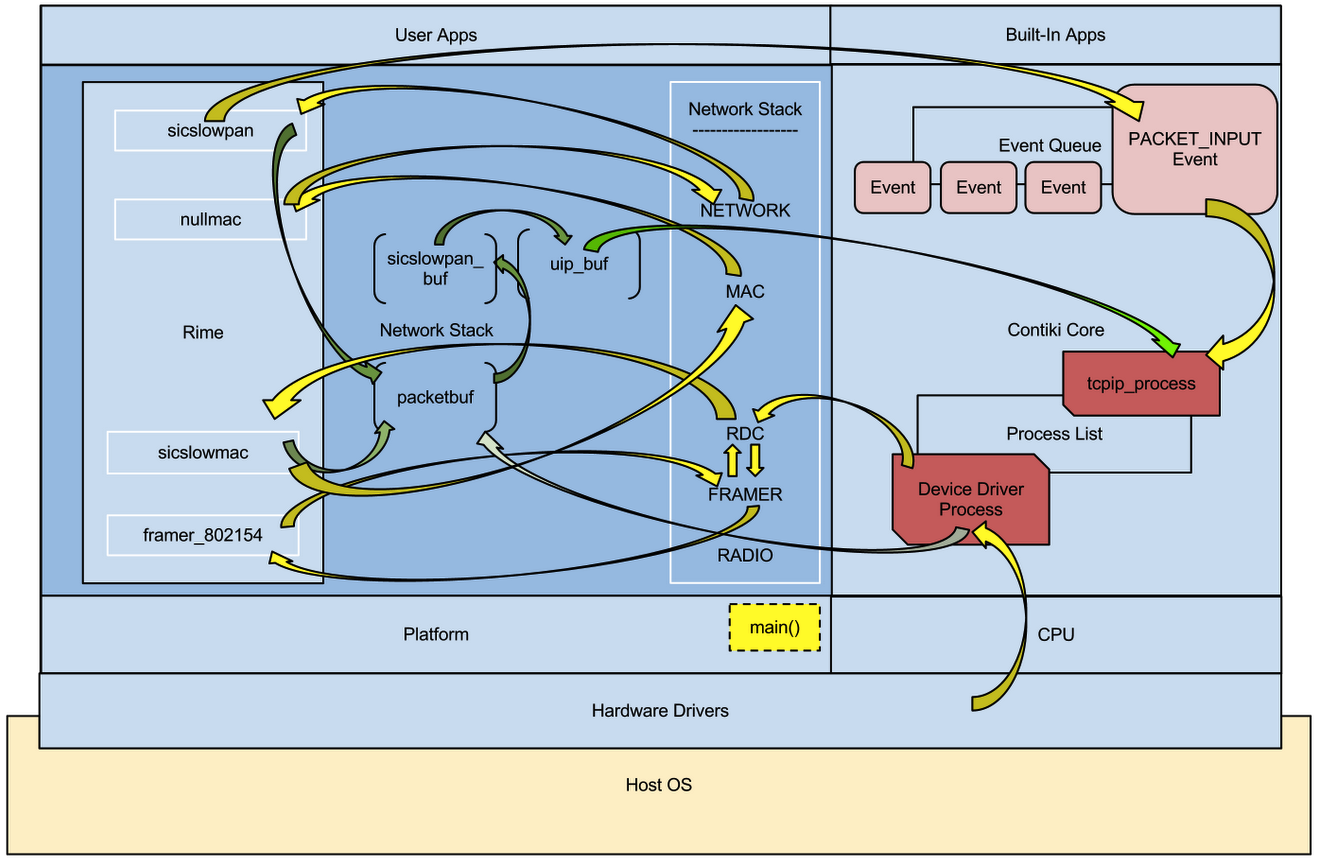
\includegraphics[width=12.5cm]{images/ch4-contiki-netstack.png}
\flcaption{Représentation fonctionnelle des dépendances au sein
de l'architecture de Contiki OS.
(Source~: \cite{BlogJUdit})}
\label{FigArchiReseauContiki}
\end{figure}

Cette complexité, combinée avec le manque de documentation (notamment
de références techniques), fait de toute tentative de contribution au code
de Contiki~--- et notamment de sa pile réseau~--- une tâche difficile,
pénible et sujette à de nombreuses erreurs.

\bigskip

En outre, comme ces difficultés sont des conséquences directes des principes
fondamentaux ayant présidé à la conception du système et de sa pile réseau,
il est difficilement envisageable de corriger ces défauts sans devoir
changer en profondeur l'architecture interne du système, ce qui
impliquerait bien évidemment des incompatibilités majeures (et donc
très probablement inacceptables pour la communauté des utilisateurs)
avec le code existant. Par conséquent, le besoin d'une documentation
technique précise, complète, détaillée et accessible est encore plus
critique.


\subsection{Fonctionnalités temps-réel insuffisantes}
\label{SubsecContikiTempsReel}

Pour implanter les protocoles avancés que nous avons décrit en section
\vref{SubsecProtoMACavances} du présent document, il est nécessaire de
gérer les évènements système (comme les interruptions) avec réactivité~---
c'est-à-dire avec un délai de latence minimal~--- et flexibilité. Ces
protocoles reposent en effet sur un \lang{timing} précis pour assurer
une synchronisation efficace entre les différents noeuds et autres
appareils appartenant aux différents réseaux de capteurs sans-fil (PANs),
permettant ainsi de faire fonctionner l'émetteur~/ récepteur radio des
noeuds seulement quand cela est nécessaire. L'émetteur~/ récepteur radio
est en effet le composant le plus gourmand en énergie dans ces noeuds,
et le mettre hors fonction est l'un des principaux moyens d'augmenter
la durée de vie de leur batterie.

Pour parvenir à une synchronisation temporelle suffisamment précise, nous
avons besoin d'une plate-forme logicielle offrant des fonctionnalités
temps-réel (c'est-à-dire garantissant que l'exécution d'une tâche donnée
se fera dans un délai respectant une échéance maximale donnée) avec une
granularité temporelle suffisamment fine.

Contiki, comme nous l'avons vu en section \vref{SubsecContikiOS}, n'est
pas à la base un système temps-réel~: le noyau est basé sur un ordonnanceur
évènementiel, basé sur du multitâche coopératif. Cet ordonnanceur ne se
déclenche qu'à intervalle fixe, pré-déterminé par une constante de
compilation. Sur les plates-formes que nous utilisons sous Contiki (les
\lang{motes} Sky/TelosB et Zolertia Z1), ce rythme de déclenchement de
l'ordonnanceur est fixé à 128~Hz, ce qui correspond à un délai de traitement
d'un évènement pouvant monter jusqu'à 8~millisecondes (8000~microsecondes),
sachant que le traitement d'une interruption fait partie des <<~évènements~>>
potentiels. Une granularité aussi large dans la réactivité du système est
clairement un problème majeur, notamment pour l'implantation de protocoles
MAC~/ RDC à hautes performances, sachant que la durée de transmission d'une
trame 802.15.4 de taille maximale (127 octets) est d'environ 4~millisecondes,
et que la durée de base d'une période de \lang{backoff} CSMA~/ CA est de
seulement 320~microsecondes.

Pour tenter de pallier ce problème, Contiki propose une fonctionnalité
dédiée à la gestion des évènements en temps-réel, nommée
\nom{\texttt{rtimer}}. Ce mécanisme permet d'outrepasser l'ordonnanceur
du noyau de Contiki, et d'utiliser un \lang{timer} matériel (c'est-à-dire
implanté comme périphérique physique dans le microcontrôleur au c{\oe}ur
du noeud) pour déclencher une fonction choisie par l'utilisateur.
Malheureusement, ce mécanisme souffre de sévères limitations~:

\begin{itemize}

\item Une seule et unique instance de \texttt{rtimer} est disponible pour
tout le système~; par conséquent, une seule tâche en temps-réel peut être
programmée ou exécutée à chaque instant. Cette limitation rend la
conception de programmes temps-réel un tant soit peu complexes~---
tel un protocole MAC~/ RDC, ou pire encore une pile réseau complète,
devant gérer simultanément plusieurs délais précis~--- plus difficile
à gérer et implémenter.

\item De plus, il est dangereux, pour la stabilité du système, d'exécuter
depuis une fonction déclenchée par \texttt{rtimer} la quasi-totalité
des fonctions de base de Contiki (c'est-à-dire~: le noyau, la pile réseau,
etc.), même de façon indirecte, car le code composant le c{\oe}ur de Contiki
n'a pas été conçu pour gérer la préemption (techniquement parlant, ces
fonctions ne sont pas <<~réentrantes~>>). Contiki est en effet basé sur
le paradigme du multitâche coopératif, tandis que \texttt{rtimer} se
comporte plutôt comme un mécanisme <<~indépendant~>>, venant avec son
propre paradigme. Seul un ensemble restreint de fonctions système définies
comme \lang{``interrupt-safe''} (par exemple~: la fonction
\texttt{process\_poll()}) peuvent être appelées en toute sécurité depuis
une <<~tâche~>> \texttt{rtimer}, l'utilisation de toute autre fonctionnalité
de Contiki conduisant de façon quasi-certaine à un plantage ou à un
comportement imprévisible du système. Cette restriction rend en pratique
le développement d'extensions temps-réel au système Contiki (via l'emploi
de \texttt{rtimer}) extrêmement difficile et limité.

\end{itemize}

Au final, et malgré l'introduction du mécanisme \texttt{rtimer}, qui est
comme nous venons de le voir extrêmement limité, il est impossible de
considérer Contiki comme un système temps-réel (même dans la définition
la plus <<~large~>> du terme).

\label{PtEchecSCosensContiki}
Une tentative d'implantation de S-CoSenS a malgré tout été réalisée
sous Contiki, mais pour les raisons citées dans la présente section
\ref{SecLimContiki}, il a été impossible de rendre celle-ci un tant soit
peu fonctionnelle. Suite à cet échec, nous avons donc définitivement
abandonné l'idée d'utiliser Contiki comme plate-forme logicielle pour
nos travaux de thèse, la présence de fonctionnalités temps-réel étant
indispensable pour pouvoir~:

\begin{itemize}

\item synchroniser de façon suffisamment précise les différents noeuds 
des WSN~;

\item ou même, ne serait-ce que pour respecter les durées des diverses
périodes et donc implanter de façon satisfaisante nos protocoles MAC~/ RDC
avancés.

\end{itemize}

%%%%%%%%%%%%%%%%%%%%%%%%%%%%%%%%%%%%%%%%%%%%%%%%%%%%%%%%%%%%%%%%%%%%%%%%%%%%%

\section{RIOT OS~: découverte et contributions}
\label{SecRIOTContrib}


\subsection{La plate-forme logicielle RIOT OS}
\label{SubSecPFRIOT}

Nous nous sommes alors intéressés à RIOT OS qui, comme indiqué dans
la section \vref{SubsecRIOTOS}, offre toutes les fonctionnalités dont
nous avons besoin pour nos développements, notamment~: un micro-noyau avec
un ordonnanceur fonctionnant selon le paradigme du multitâche préemptif,
ainsi que la possibilité d'utiliser les \lang{timers} matériels du
microcontrôleur, et ce avec une granularité au moins aussi fine
que le permettent ces \lang{timers} matériels.

Sur les premiers matériels que nous avons utilisés (TelosB et Z1), cette
granularité est d'environ $30,5~\mu$s (la fréquence des \lang{timers}
étant comme nous l'avons vu de 32~KHz). Une telle granularité est tout
à fait satisfaisante pour nos travaux.

RIOT OS a historiquement d'abord été développé~--- sous le nom de
<<~Feuerware~>>~--- sur des appareils à architecture ARM aujourd'hui
obsolètes (famille ARM7\-TDMI), puis a été porté sur des microcontrôleurs
plus récents (ARM Cortex-M) ainsi que d'autres architectures (MSP430
puis plus récemment Atmel AVR).

Toutefois, lorsque nous avons commencé à travailler avec RIOT (début 2014),
le portage sur MSP430 n'était pas aussi bien débogué que le code ARM, et
était souvent victime de plantages.


\subsection{Contributions au projet RIOT OS}
\label{SubSecContribRIOT}

Nos contributions, lors de cette première partie de nos travaux de thèse
sur RIOT OS, peuvent ainsi être résumées en les points suivants~:

\subsubsection{Gestion des erreurs fatales}
\label{ParRIOTCorePanic}

Nous avons d'abord \emph{ajouté des fonctionnalités de déboguage
au noyau de RIOT OS, et notamment un mécanisme destiné à prendre en charge
les erreurs fatales} \cite{PRriotPanic}.

\smallskip

Cet ajout s'est inspiré de la fonction noyau \texttt{panic()} bien
connue dans le monde des systèmes Unix et dérivés. Cette fonction,
en générale interne au noyau système, sert à gérer les erreurs fatales,
en arrêtant le système, en essayant souvent de fournir le maximum
d'informations concernant le problème survenu, et si possible en
limitant les risques de dommages (notamment aux données stockées
sur le système, voire dans certains rares cas au matériel).
Cette procédure d'arrêt <<~en catastrophe~>> du système est nommée,
dans le monde <<~unixien~>>, \emph{``kernel panic''}.

Son équivalent dans les systèmes Microsoft (Windows) et autres
(OS/2, iOS) est le \lang{``Screen of Death''}~--- le plus souvent bleu
ou noir (d'où l'acronyme BSOD).

Dans ces systèmes destinés à l'informatique <<~lourde~>> (des PC
aux macro-ordinateurs), \texttt{panic()} est une fonction interne
au noyau, car ce dernier s'appuie sur des dispositifs matériels de
gestion de la mémoire (à savoir une \nom{MMU}~: unité de gestion
de mémoire), rendant la majorité des programmes~--- nommément
tous ceux ne s'exécutant pas en <<~mode privilégié~>> ou <<~espace
mémoire noyau~>>, c'est-à-dire normalement toutes les applications
lancées par l'utilisateur~--- incapables d'endommager les structures
de données et autres ressources vitales pour l'exécution du système.
Ces programmes ne manipulent en effet, via le fonctionnement d'une MMU
en mode <<~non privilégié~>> ou <<~utilisateur~>>, que des adresses
<<~logiques~>> (également parfois appelées adresses <<~linéaires~>> ou
<<~virtuelles~>>) au sein d'un espace mémoire virtuel propre à chaque
programme en cours d'exécution~; la manipulation réelle des adresses
physiques sous-jacentes se faisant exclusivement au travers de la MMU et
de ses stricts mécanismes de sécurité et de séparation des espaces mémoires,
configurés par le noyau. Un programme en <<~mode utilisateur~>> est ainsi
normalement incapable de corrompre tout espace mémoire différent du sien,
que ce soit celui des autres applications, ou \lang{a fortiori} celui du
c{\oe}ur du système.
Une erreur fatale ne peut par conséquent normalement survenir que lorsqu'un
problème survient dans le code s'exécutant en <<~mode privilégié~>>
(c-à-d~: code du noyau lui-même, ou pilotes de périphériques).

\smallskip

Dans les systèmes embarqués, il n'y a pas de MMU~: tout au plus
une \nom{MPU} (unité de protection mémoire) offrant une limitation d'accès
à certaines zones mémoire selon le mode (privilégié ou non).

Malheureusement, toutes les architectures de processeurs embarqués
n'offrent pas ce mécanisme de MPU~: il n'existe pas dans les
architectures AVR et MSP430, et n'est qu'optionnel pour les ARM
(notamment Cortex-M), beaucoup de microcontrôleurs implantant cette
dernière architecture font ainsi l'impasse sur ce mécanisme.

Il faut également préciser que les applications (souvent uniques) d'un
système embarqué ayant régulièrement besoin d'accéder directement aux
ressources matérielles~--- notamment pour des raisons d'efficacité~---
beaucoup d'entre elles sont, pour des raisons de simplicité, programmées
pour fonctionner exclusivement en mode privilégié, rendant ainsi tout
mécanisme de MPU inopérant.

Pour toutes ces raisons RIOT OS (du moins dans les versions \texttt{2013.08}
à \texttt{2015.12} incluses, que nous avons utilisées dans le cadre de
la présente thèse) n'utilise aucune MPU, même sur les architectures
où un tel mécanisme est présent.

\smallskip

Ainsi, nous avons dès le départ clairement déterminé qu'une fonction
de gestion des erreurs fatales ne saurait être un mécanisme interne
au noyau de RIOT, mais devrait être une primitive système explicitement
offerte par ce dernier à l'ensemble du code~--- noyau, pilotes et
applications système. Cette fonction a été, après discussion avec le
reste de l'équipe de développement, nommée \nom{\texttt{core\_panic()}}.

Nous avons voulu reproduire le maximum des possibilités offertes
par les procédures équivalentes des systèmes pour l'informatique
<<~classique~>> (PC et autres)~: les systèmes <<~plantés~>> peuvent
ainsi être <<~gelés~>> pour faciliter leur déboguage durant les phases de
développement~; ou, en production, être au contraire immédiatement
redémarrés, réduisant ainsi l'indisponibilité d'un appareil fonctionnant
sous RIOT au minimum~; le choix entre les deux comportements se fait
via une constante de compilation.

Cette contribution s'est vue décerner le titre de \emph{``PR of the
month''} pour le mois de février 2014 par le projet RIOT OS.

Cette contribution utilise une autre de nos contributions implantant
une primitive de redémarrage (fonction \texttt{reboot()}) au noyau de RIOT
pour le mode production \cite{PRriotEnh5} \cite{PRriotEnh3}.

\subsubsection{Portage sur une nouvelle plate-forme matérielle}
\label{ParRIOTZolertiaZ1}

Nous avons \emph{porté RIOT OS sur la Zolertia Z1} \cite{PRriotPortZ1},
qui est rappelons-le une \lang{mote} basée sur l'architecture MSP430,
utilisée de façon industrielle (notamment avec Contiki).

\smallskip

Dans la plupart des systèmes d'exploitation visant la portabilité (comme
par exemple Unix~/ Linux, ou les différentes déclinaisons de Microsoft
Windows NT), la majorité du code du système est conçue de façon générique,
c'est-à-dire avec une structure et un fonctionnement indépendants de la
plate-forme matérielle sous-jacente.

Le code dépendant de la plate-forme est réduit au minimum, et se charge
d'offrir au reste (très majoritaire) du système une API prédéfinie
lui permettant d'accéder au matériel tout en <<~ignorant~>> ces
spécificités. L'ensemble restreint de ce code dépendant des plates-formes
matérielles et cachant les disparités de ces dernières est nommé
\nom{couche d'abstraction matérielle} (\nom{HAL~:} \lang{Hardware
Abstraction Layer}).

\smallskip

RIOT OS, comme la plupart des systèmes portables, est conçu selon ce modèle
employant une couche d'abstraction matérielle. Un portage de RIOT OS sur un
nouveau matériel consiste donc à créer une variante de cette couche capable
de gérer la nouvelle plate-forme matérielle visée.

Cette couche d'abstraction matérielle se charge notamment, sous RIOT OS,
d'assurer le support des changements de contexte lors des basculements entre
tâches (en support à l'ordonnanceur), l'implantation des fonctions concernant
les \lang{timers} ou les différents périphériques implantés au sein du
microcontrôleur, ainsi que l'accès aux entrées~/ sorties (GPIO). Du point
de vue de l'implantation, la couche d'abstraction matérielle peut être vue
comme un ensemble de pilotes (\lang{``drivers''}) chargés d'implanter l'API
prédéfinie entre cette couche et le reste du système d'exploitation~;
ces pilotes doivent en général lire et écrire les registres matériels
de façon adéquate, en fonction des opérations demandées.

\smallskip

La couche d'abstraction matérielle de RIOT OS se divise fonctionnellement
en plusieurs sous-parties~:

\begin{enumerate}

\item Une partie <<~\emph{MCU}~>> destinée à supporter les différentes
architectures de microcontrôleurs visées. Cette partie prend en charge les
fonctionnalités spécifiques de chaque architecture de microcontrôleur,
elle regroupe ainsi le code commun entre plates-formes matérielles basées sur
des microcontrôleurs similaires (ARM7, Cortex-M, MSP430, AVR...). Dans notre
cas, le code commun destiné à supporter l'architecture MSP430 existait déjà~:
nous n'avons ainsi pas eu à nous occuper de cette partie MCU pour effectuer
notre portage.

Cette partie de la couche d'abstraction matérielle se charge notamment des
opérations liées aux registres et mécanismes du c{\oe}ur du microcontrôleur~:
par exemple de l'implantation des changements de contexte lors des
basculements entre tâches.

\item Une partie <<~\emph{périphériques}~>> regroupant des pilotes génériques
pour des circuits intégrés communs, susceptibles d'être retrouvés dans
plusieurs matériels différents~: c'est le cas des émetteurs~/ récepteurs
radio, des capteurs environnementaux divers (ex.~: température, humidité,
etc.). Nous n'avons pas non plus eu besoin pour ce travail de portage
d'intervenir directement sur cette partie.

Ces pilotes <<~génériques~>> sont ensuite exploités de façon adéquate par
du code <<~de liaison~>> (\lang{``glue''} en anglais) spécifique~---
impliquant souvent un bus géré par le microcontrôleur comme SPI ou
I\textsuperscript{2}C~--- permettant leur mise en {\oe}uvre sur chaque
plate-forme matérielle différente. Ce code de liaison est implanté dans
la dernière partie de la couche d'abstraction matérielle décrite ci-dessous.

\item Une partie <<~\emph{plate-forme}~>> regroupant les éléments
véritablement spécifiques à une plate-forme matérielle donnée. Elle
regroupe notamment les pilotes du matériel purement spécifique à une
plate-forme donnée, ainsi que le code <<~de liaison~>> (\lang{``glue''})
avec les parties plus génériques de la couche d'abstraction matérielle.
C'est cette partie que nous avons créée pour le support spécifique de
la plate-forme matérielle Zolertia Z1.

Ce travail, comme nous l'avons dit ci-dessus, a principalement consisté
à implanter des pilotes~--- notamment pour les \lang{timers} matériels,
le port série~/ USB (UART) et les GPIO~--- ainsi qu'une fonction
d'initialisation adéquate, principalement en manipulant les registres
adéquats des périphériques. Nous avons également créé le code de liaison
nécessaire avec le pilote pré-existant pour l'émetteur~/ récepteur radio
CC2420 qui équipe cette \lang{mote}, via la configuration adéquate du bus
SPI du microcontrôleur.

\end{enumerate}

\subsubsection{Déboguage des portages sur MSP430}
\label{ParRIOTDebugMSP430}

Nous avons \emph{débogué les portages de RIOT OS sur MSP430}~--- plus
précisément~: la portion spécifique de la couche d'abstraction matérielle
de l'ordonnanceur chargée de traiter les changements de contexte
lors des basculements entre tâches \cite{PRriotFix2MSP430}
\cite{PRriotFix3MSP430} \cite{PRriotFix1MSP430}~--- rendant ainsi RIOT
robuste et prêt à l'usage en production sur les appareils basés sur
l'architecture MSP430.

\smallskip

Pour effectuer un tel déboguage de façon efficace, il est nécessaire~:

\begin{itemize} 

\item Soit de disposer de la possibilité de faire appel à des fonctions
de déboguage directement présentes dans le matériel, en général rendues
accessibles via le protocole JTAG. La plupart des microcontrôleurs
sur lesquels sont basées les \lang{motes} offrent des broches spécifiques
dédiées à ce mécanisme de déboguage~; il faut néanmoins que la \lang{mote}
elle-même rende ces signaux accessibles via un port quelconque, ce qui
n'est pas évident. En outre, un adaptateur JTAG, presque toujours spécifique
de l'architecture du microcontrôleur à déboguer, est nécessaire pour relier
le matériel à déboguer et le PC~/ station de travail du développeur.
Enfin, le protocole JTAG ne permet sauf exception que d'agir sur le
microcontrôleur lui-même, pas d'avoir accès aux circuits annexes comme
les émetteurs~/ récepteurs radio autonomes (tel le CC2420 de la Zolertia
Z1).

\item Soit de disposer d'un émulateur suffisamment fiable, et fidèle au
fonctionnement réel du matériel sur lequel le programme à déboguer doit
s'exécuter. Celui-ci peut alors offrir des fonctions de déboguage avancées,
comparables à ce qu'offrent les environnement de développement pour PC.
Un tel émulateur est MSPSim \cite{MSPSim}, fourni en standard avec le
simulateur de réseaux de capteurs sans-fil Cooja \cite{Cooja} du projet
Contiki, lequel émule plusieurs \lang{motes} basées sur l'architecture
MSP430, notamment les TelosB~/SkyMotes et~--- surtout~--- la Zolertia Z1.

\end{itemize}

\smallskip

Les problèmes qui touchaient les portages de RIOT OS sur MSP430 étaient mal
reproductibles, car imprévisibles (bien que fréquents)~: leur déclenchement
n'ayant pu être lié ni à l'utilisation d'une certaine fonctionnalité, ni au
passage dans une portion spécifique du code de RIOT, ni à l'écoulement d'un
certain délai. Dans ces conditions, il est très difficile de trouver la
cause d'un problème, même en utilisant les meilleurs outils de déboguage.

Pour trouver la raison principale des plantages de RIOT OS sur MSP430,
nous avons eu recours à la technique dite de \nom{traçage des instructions~:}
cette technique consiste à enregistrer chaque instruction exécutée par
le matériel lors du fonctionnement du code défectueux (soit pour toute
la durée d'exécution, soit pour un intervalle de temps donné). Au final,
l'utilisation de cette technique permet d'obtenir un \lang{listing}
assembleur précis, reproduisant fidèlement les instructions élémentaires
exécutées lors du déroulement du programme.

Employer la technique de traçage avec un débogueur matériel nécessite
l'emploi d'un adaptateur JTAG haut de gamme, disposant de la quantité
de mémoire nécessaire pour enregistrer les instructions exécutées. De tels
adaptateurs sont coûteux, et n'existent pas pour toutes les architectures~:
l'unique adaptateur JTAG MSP430 vendu par Texas Instruments ne dispose pas
d'une telle fonctionnalité.

À l'inverse, \emph{le couple Cooja~/ MSPSim offre une telle fonctionnalité
de traçage des instructions}. Nous avons donc utilisé cette possibilité,
qui nous a finalement permis de découvrir la source de la principale cause
d'instabilité sur MSP430, à savoir~: l'inactivation trop tardive des
interruptions pendant le changement de contexte de tâche, permettant
à une interruption de stopper la sauvegarde du contexte de la tâche
en cours d'arrêt, ce qui bien évidemment corrompait le plus souvent
le contexte sauvegardé, provoquant le plantage du système lors de la
réactivation de la tâche touchée. Cette réactivation intervenant de façon
non déterministe, en fonction de la charge du système et de sa gestion par
l'ordonnanceur, on comprend ainsi pourquoi ces plantages intervenaient
sans raison \lang{a priori} discernable. Nous avons donc, grâce aux
fonctions avancées de déboguage et traçage de MSPSim, pu comprendre
le principal problème et y apporter une solution. Cette solution consiste
à corriger l'ordre des instructions dans la fonction \texttt{thread\_yield()},
faisant partie de la partie de la couche d'abstraction matérielle de RIOT
gérant l'architecture MSP430~: les interruptions sont désormais désactivées
dès le début de la fonction, \emph{avant} de commencer à sauvegarder le
contexte du \lang{thread} en cours de suspension, et ne sont réactivées
(si nécessaire) qu'une fois le contexte du \lang{thread} à relancer
totalement restauré \cite{PRriotFix2MSP430}.

La correction de deux autres problèmes liés à la gestion des \lang{timers}
des MSP430 par cette même couche d'abstraction matérielle, plus simples à
comprendre et à résoudre, a permis d'achever la fiabilisation des portages
de RIOT OS~:
\begin{enumerate}
\item la correction de l'implantation de la fonction \texttt{hwtimer\_spin()},
en évitant que ne soit calculée une valeur-cible impossible à atteindre
par le compteur du \lang{timer} voulu \cite{PRriotFix1MSP430}~;
\item l'abandon de la prise en charge de délais supérieurs à $2^{16}$
\lang{``ticks''} de \lang{timers} pour l'implantation du mécanisme
\texttt{hwtimer} sur MSP430 \cite{PRriotFix3MSP430}.
\end{enumerate}
Ces deux erreurs étaient dues à la différence de type entre les valeurs
calculées par les implantations des fonctionnalités liées aux mécanismes
temps-réel de \texttt{hwtimer}~--- utilisant des entiers~32 bits~--- et
les compteurs des \lang{timers} matériels des MSP430~--- qui ne sont
que des entiers de 16~bits \footnotemark[2].

\footnotetext[2]{Ce type de problèmes et limitations a conduit au
remplacement du mécanisme \texttt{hwtimer} par le module \texttt{xtimer},
de conception différente et de plus haut niveau (comme vu en section
\vref{SubsecRIOTOS}), et donc normalement moins vulnérable vis-à-vis
de telles difficultés d'implantation.}

\medskip

La possibilité de faire fonctionner RIOT sur MSP430 permet donc
\emph{d'exécuter des applications basées sur ce système dans le simulateur
Cooja~/ MSPSim. Cela facilite grandement la rapidité et l'efficacité
du développement de telles applications.} Nous venons notamment de le
démontrer, le déboguage de la couche d'abstraction matérielle de RIOT pour
les microcontrôleurs MSP430 aurait probablement été extrêmement difficile
sans ses fonctionnalités de déboguage et notamment de traçage.

Au final, on voit qu'un émulateur \emph{de qualité} peut se révèler un outil
de développement et déboguage extrêmement précieux, en complément des
débogueurs matériels, ou même en remplacement de ces derniers, lorsque
ceux-ci sont trop coûteux ou~--- surtout~!~--- n'offrent pas les
fonctionnalités nécessaires comme cela a été le cas ici. Bien évidemment,
\emph{l'émulateur en question, pour remplir ce rôle, doit être très fidèle
au fonctionnement du matériel émulé pour être utile}. Dans ce cas précis,
MSPSim s'est révélé tout à fait à la hauteur quant à l'émulation du c{\oe}ur
du microcontrôleur MSP430 (au niveau duquel se produisait le bogue à
corriger).

\subsubsection{Contributions diverses}
\label{ParRIOTContribDiverses}

D'autres contributions ont été apportées, ayant eu un impact moindre sur
l'avancée du projet RIOT OS. Celles-ci se divisent en deux groupes~:

\begin{enumerate}

\item les contributions de \emph{déboguage}~:
\begin{itemize}
\item réparation du mécanisme d'échange de données entre microcontrôleur et
émetteur~/ récepteur radio sur Zolertia Z1, en corrigeant le test vérifiant
la bonne émission d'un octet sur le bus SPI (retrait d'une négation logique
erronée) \cite{PRriotDebug9},
\item correction de diverses erreurs dans le pilote pour l'émetteur~/
récepteur radio CC2420 au niveau de l'implantation~: correction d'une
constante \cite{PRriotDebug3}, de la gestion des adresses et du PAN ID
\cite{PRriotDebug2}, de la gestion du bus SPI pour communiquer avec
la radio (notamment la fonction \texttt{cc2420\_do\_send()})
\cite{PRriotDebug7}, et dans la détermination du CCA (mauvaise gestion
du bus SPI dans l'implantation de cette fonctionnalité) \cite{PRriotDebug8},
\item correction d'erreurs intermittentes concernant les \lang{timers}
matériels des MCU MSP430, notamment en déclarant certaines variables
\texttt{volatile}s au sein de l'implantation \cite{PRriotDebug4},
\item fiabilisation des mécanismes de gestion des interruptions sur
architecture MSP430, en ajoutant un <<~délai d'attente~>> (instruction
\texttt{NOP}) après l'activation ou la désactivation générale des
interruptions au niveau du microcontrôleur (comme recommandé dans les
manuels de TI), et en s'assurant que les interruptions sont bien activées
avant l'entrée en mode basse consommation (pour pouvoir sortir de ce
dernier) \cite{PRriotDebug10},
\item fiabilisation de l'alignement du pointeur de pile (registre SR)
lors de la création de threads \cite{PRriotDebug1},
\item fiabilisation du processus de \lang{flashage} des applications sur
ARM Cortex-M3, en forçant un effacement de la mémoire et un \lang{reset}
avant le lancement du processus de \lang{flashage} proprement dit
\cite{PRriotDebug6},
\item correction et la fiabilisation de la fonction d'attente active via
l'utilisation des timers matériels (\texttt{hwtimer\_spin()}), en modifiant
l'implantation pour la rendre plus simple, compréhensible et fiable
\cite{PRriotDebug5}~;
\end{itemize}

\item les contributions \emph{apportant des améliorations et fonctionnalités
supplémentaires}~:
\begin{itemize}
\item amélioration de l'API et des fonctionnalités des pilotes des
émetteurs~/ récepteurs radio \cite{PRriotEnh12} \cite{PRriotEnh10}
\cite{PRriotEnh11} \cite{PRriotEnh7} \cite{PRriotEnh6},
\item gestion des modes <<~basse énergie~>> des MCU MSP430
\cite{PRriotEnh2},
\item réorganisation et simplification des fichiers d'entête
(\texttt{xxx.h}) pour la partie MSP430 de la couche d'abstraction
matérielle \cite{PRriotEnh1},
\item augmentation du nombre d'instances de \lang{timers} matériels
(\texttt{hwtimer}s) utilisables sur MSP430 \cite{PRriotEnh9},
\item ajout d'une primitive de redémarrage (fonction \texttt{reboot()})
au noyau de RIOT (notamment employée par la gestion des erreurs fatales
pour réactiver au plus vite un système planté en mode production, voir
\vref{ParRIOTCorePanic}) \cite{PRriotEnh5} \cite{PRriotEnh3},
\item définition d'attributs de fonction <<~portables~>> \cite{PRriotEnh4},
\item possibilité pour un thread d'envoyer un message à lui-même
(pour permettre par exemple les appels de fonction retardés~---
\lang{``deferred procedure calls''} en anglais) \cite{PRriotEnh8},
\item ajout d'une option pour la gestion du \lang{``CCA threshold''}
dans la nouvelle pile gnrc \cite{PRriotEnh13}.
\end{itemize}

\end{enumerate}

\medskip

Notons que toutes ces contributions ont été revues et acceptées par
l'équipe de développement de RIOT, qui les a intégrées dans le source
\lang{``master''} du système~: elles font donc maintenant partie du
système de base \footnotemark[3].

\footnotetext[3]{Les changements récents dans la pile réseau et la gestion
des \lang{timers} du système RIOT ont toutefois rendu obsolète le code
apporté par certaines de ces contributions~; néanmoins, les fonctionnalités
correspondantes ont en général été réimplantées d'une façon différente
et adéquate dans les nouvelles versions de RIOT OS.}

\bigskip

Grâce à toutes ces avancées, nous avons maintenant une plate-forme
logicielle robuste et offrant les fonctionnalités nécessaires pour
développer nos protocoles MAC~/ RDC à hautes performances~--- notamment
ceux basés sur l'ordonnancement temporel (TDMA).
C'est pourquoi nous avons implanté et testé S-CoSenS sur RIOT OS lors des
expériences que nous décrirons au chapitre \vref{ChProtocolesMAC}.


\subsection{\'Evolution du système RIOT OS}
\label{SubSecEvoRIOT}

Depuis que lesdites expériences du chapitre \ref{ChProtocolesMAC} ont
été menées, RIOT OS a continué à évoluer de façon rapide et profonde~---
et tout particulièrement sa pile réseau, qui a fait l'objet d'une refonte
totale. Cette évolution étant potentiellement amenée à modifier, non
seulement les résultats des expériences citées ci-dessus, mais aussi
ceux des travaux présentés plus loin au chapitre \vref{ChValidation}
(et notamment à influer sur les problèmes détaillés dans ce dernier
chapitre), nous allons maintenant procéder à une analyse détaillée
et critique de cette nouvelle pile réseau.

%%%%%%%%%%%%%%%%%%%%%%%%%%%%%%%%%%%%%%%%%%%%%%%%%%%%%%%%%%%%%%%%%%%%%%%%%%%%%

\section{La nouvelle pile réseau de RIOT~: une analyse critique}
\label{SecGnrcRIOT}

Nous décrivons, dans les sections \vref{ParAPIRadioContiki} puis
\vref{SubsecAPIRadioExt}, notre mécanisme de <<~capacités~>> permettant
de profiter de façon portable des spécificités des émetteurs~/ récepteurs
radio des \lang{``motes''}, grâce à des fonctions génériques de gestion
d'un ensemble varié et extensible de constantes et paramètres.
Un mécanisme de ce type est désormais intégré dans Contiki 3.0
\cite{Contiki3Annonce} (suite en partie et de façon indirecte à certaines
de nos contributions). Une évolution similaire a eu lieu pour RIOT OS.

En effet, pendant que nous tentions d'effectuer nos travaux
et subissions les problèmes techniques détaillés dans la section
\vref{SecTravauxMiseOeuvre}, RIOT OS a durant l'année 2015 subi une
refonte de sa pile réseau~--- une pile réseau nouvelle génération,
se voulant générique (\nom{<<~gnrc~>>}), est apparue, sur laquelle
nous allons nous pencher dans la présente section.

Compte-tenu du sujet de la présente thèse, nous nous focaliserons sur les
couches les plus basses (physique~/ pilote radio, et MAC~/ RDC) de cette
nouvelle pile.


\subsection{Description}
\label{SubsecDescrGnrc}

L'API des pilotes pour les émetteurs~/ récepteurs radio de la nouvelle
pile <<~gnrc~>> a repris le principe de ce que nous avons appelé le
mécanisme de <<~capacités~>>, implantant pour les pilotes radio
un ensemble, extrêmement réduit, de fonctions génériques, dont le
détail est donné en table \vref{TblGnrcFnct}. (Notons toutefois que nous
n'avons pas pu participer à l'implantation de ces nouveaux pilotes,
ni à la conception de la nouvelle pile <<~gnrc~>>, étant monopolisés
par nos propres travaux.)


\begin{table}[!hbt]
\centering

\begin{tabular}{|l|p{9cm}|}
\hline
\textbf{Nom} & \textbf{Rôle} \\
\hline
\texttt{send\_data()} & Envoie une trame via l'émetteur~/ récepteur radio \\
\hline
\texttt{add\_event\_callback()} & Ajoute une fonction \lang{``callback''}
                                  pour la gestion des évènements remontés
                                  par le pilote radio donné \\
\hline
\texttt{rem\_event\_callback()} & Retire une fonction \lang{``callback''}
                                  pour la gestion des évènements remontés
                                  par le pilote radio donné \\
\hline
\texttt{get()} & Lit la valeur courante d'une option de configuration
                 d'un pilote radio donné \\
\hline
\texttt{set()} & Définit la valeur courante d'une option de configuration
                 d'un pilote radio donné \\
\hline
\texttt{isr\_event()} & Fonction \lang{``callback''} pouvant être
                        appelée par une couche supérieure de la pile
                        réseau, pour signaler un évènement au pilote
                        radio (cet <<~évènement~>> étant actuellement
                        une valeur numérique totalement arbitraire) \\
\hline
\end{tabular}

\flcaption{Liste des fonctions des pilotes radio nouvelle génération
(<<~gnrc~>>).}
\label{TblGnrcFnct}
\end{table}


Les <<~évènements~>> pour lesquels il est possible de définir des
\lang{``callbacks''} sont listés en table \vref{TblGnrcEvnt}.
(Le déclenchement ou non de ces \lang{``callbacks''} se fait en fonction
de la valeur des options \texttt{NETOPT\_*\_*\_IRQ} définies en table
\vref{TblGnrcCapabOpt}.)


\begin{table}[!htb]
\centering

\begin{tabular}{|l|p{8cm}|}
\hline
\textbf{Nom} & \textbf{Signification} \\
\hline
\texttt{NETDEV\_EVENT\_RX\_STARTED} & Début de réception d'une trame (SFD) \\
\hline
\texttt{NETDEV\_EVENT\_RX\_COMPLETE} & Réception d'une trame terminée~:
                                       analyse possible du contenu \\
\hline
\texttt{NETDEV\_EVENT\_TX\_STARTED} & Début de transmission d'une trame \\
\hline
\texttt{NETDEV\_EVENT\_TX\_COMPLETE} & Fin de transmission d'une trame \\
\hline
\end{tabular}

\flcaption{Liste des évènements radio interceptables (<<~gnrc~>>).}
\label{TblGnrcEvnt}
\end{table}


Les différentes options pouvant être réglées par les fonctions \texttt{get()}
et \texttt{set()} sont listées dans la table \vref{TblGnrcCapabOpt}.


\begin{table}[!p]
\centering

\small
\begin{tabular}{|l|p{9cm}|}
\hline
\textbf{Identifiant} & \textbf{Signification} \\
\hline
\texttt{NETOPT\_CHANNEL} & Canal (fréquence) utilisée
                          par l'émetteur~/ récepteur radio \\
\hline
\texttt{NETOPT\_IS\_CHANNEL\_CLR} & Vérifie si le médium radio est disponible
                                 (\lang{``Clear Channel Assessment''}) \\
\hline
\texttt{NETOPT\_ADDRESS} & Définit l'adresse <<~courte~>> (intra-PAN,
                          16 bits) de la radio \\
\hline
\texttt{NETOPT\_ADDRESS\_LONG} & Définit l'adresse <<~longue~>> (64 bits pour
                               le 802.15.4) de la radio \\
\hline
\texttt{NETOPT\_ADDR\_LEN} & Taille de l'adresse longue de la radio
                           (normalement 64 bits pour le 802.15.4) \\
\hline
\texttt{NETOPT\_SRC\_LEN} & Taille de l'adresse source à utiliser
                          pour la radio \\
\hline
\texttt{NETOPT\_NID} & Définit l'identifiant du réseau (PAN ID) \\
\hline
\texttt{NETOPT\_IPV6\_IID} & Définit l'adresse IPv6 de l'interface réseau
                           (RFC 4291, section 2.5.1) \\
\hline
\texttt{NETOPT\_TX\_POWER} & Définit la puissance d'émission
                           de la radio en dBm \\
\hline
\texttt{NETOPT\_MAX\_PACKET\_SIZE} & Définit la taille maximale d'une trame
                                  (normalement 127 octets pour le 802.15.4) \\
\hline
\texttt{NETOPT\_PRELOADING} & Active ou désactive la possibilité de
                             pré-charger le \lang{``buffer''} de
                             transmission de la radio sans lancer
                             immédiatement l'émission de la trame \\
\hline
\texttt{NETOPT\_PROMISCUOUSMODE} & Active ou désactive le mode <<~moniteur~>>
                                  (\lang{``promiscuous''}) \\
\hline
\texttt{NETOPT\_AUTOACK} & Active ou désactive l'acquittement automatique
                          des trames reçues par la radio \\
\hline
\texttt{NETOPT\_RETRANS} & Nombre maximal de retransmissions en mode CSMA/CA \\
\hline
\texttt{NETOPT\_PROTO} & Type de protocole (6LoWPAN, IPv6, TCP, UDP...)
                        pour la couche voulue \\
\hline
\texttt{NETOPT\_STATE} & \'Etat de la radio, à choisir parmi~:
                        \begin{itemize}
                        \item \texttt{NETOPT\_STATE\_OFF}~: hors tension
                        \item \texttt{NETOPT\_STATE\_SLEEP}~: mode inactif
                              basse consommation
                        \item \texttt{NETOPT\_STATE\_IDLE}~: en écoute
                              (passive)
                        \item \texttt{NETOPT\_STATE\_RX}~: réception en cours
                        \item \texttt{NETOPT\_STATE\_TX}~: transmission en
                              cours / déclenche l'émission d'une trame
                              préchargée
                        \item \texttt{NETOPT\_STATE\_RESET}~: provoque
                              une réinitialisation de la puce radio
                        \end{itemize} \\
\hline
\texttt{NETOPT\_RAWMODE} & Active ou désactive l'analyse automatique des
                          trames reçues \\
\hline
\texttt{NETOPT\_RX\_START\_IRQ} & Active ou désactive le déclenchement d'une
                               interruption au début d'une réception (SFD) \\
\hline
\texttt{NETOPT\_RX\_END\_IRQ} & Active ou désactive le déclenchement d'une
                             interruption lors de la réception d'une trame
                             complète \\
\hline
\texttt{NETOPT\_TX\_START\_IRQ} & Active ou désactive le déclenchement d'une
                               interruption au début d'une transmission \\
\hline
\texttt{NETOPT\_TX\_END\_IRQ} & Active ou désactive le déclenchement d'une
                             interruption à la fin de la transmission
                             d'une trame \\
\hline
\texttt{NETOPT\_AUTOCCA} & Active ou désactive la vérification automatique
                          de la disponibilité du médium radio
                          (\lang{``Clear Channel Assessment''})
                          par l'émetteur~/récepteur radio au début
                          d'une transmission \\
\hline
\end{tabular}

\flcaption{\small Liste des options~--- <<~capacités~>> potentielles~---
des émetteurs~/ récepteurs radio (<<~gnrc~>>).}
\label{TblGnrcCapabOpt}
\end{table}


Les fonctions présentées en table \vref{TblGnrcFnct} signalent
la survenue d'erreurs en retournant les valeurs d'erreurs (toujours
négatives) listées en table \vref{TblGnrcErr}.


\begin{table}[htb]
\centering

\begin{tabular}{|l|p{10cm}|}
\hline
\textbf{Nom} & \textbf{Signification} \\
\hline
\texttt{-ENODEV}    & Tentative d'accès à un pilote radio
                      \texttt{gnrc\_netdev\_t} invalide
                      (toutes les fonctions) \\
\hline
\texttt{-ENOMSG}    & Tentative d'envoi d'une trame invalide
                      (fonction \texttt{send\_data()}) \\
\hline
\texttt{-EOVERFLOW} & Le \lang{buffer} chargé de contenir la trame à
                      envoyer, ou les données du paramètre à lire est
                      trop petit (fonctions \texttt{send\_data()}
                      et \texttt{get()})\\
\hline
\texttt{-ENOBUFS}   & Le nombre maximal de fonctions \lang{``callbacks''}
                      pour un pilote radio donné est dépassé
                      (fonction \texttt{add\_event\_callback()}) \\
\hline
\texttt{-ENOENT}    & La fonction \lang{``callback''} à retirer n'a pas
                      été enregistrée auparavant
                      (fonction \texttt{rem\_event\_callback()})\\
\hline
\texttt{-ENOTSUP}   & Option non supportée par ce pilote radio
                      (fonctions \texttt{get()} et \texttt{set()}) \\
\hline
\texttt{-ECANCELED} & Erreur interne du pilote radio
                      (fonctions \texttt{get()} et \texttt{set()}) \\
\hline
\texttt{-EINVAL}    & Valeur invalide pour l'option transmise
                      (fonction \texttt{set()}) \\
\hline
\end{tabular}

\flcaption{Liste des erreurs potentiellement renvoyées (<<~gnrc~>>).}
\label{TblGnrcErr}
\end{table}


(Notons que les tables \vrefrange{TblGnrcFnct}{TblGnrcErr} représentent
l'état d'avancement de la pile <<~gnrc~>> au moment où nous écrivons
ces lignes~--- début septembre 2015. Cette pile étant toujours  à l'heure
actuelle l'objet d'un développement rapide et poussé, le contenu de ces
tables ne sera sans doute plus exhaustif au moment où ce manuscrit
de thèse sera lu.)

\bigskip

Le pilote radio amélioré, implantant notre concept de <<~capacités~>>,
dont nous discuterons en section \vref{SubsecAPIRadioExt} est donc déjà
obsolète, et ne sera pas intégré au code de RIOT OS.

En effet, un nouveau type de pilote radio, nommé \texttt{gnrc\_netdev\_t},
a été créé~; toutes les fonctions de la nouvelle API <<~gnrc~>> travaillent
avec des instances de ce type.

Un effort pour convertir tous les pilotes radio de RIOT à l'API de ce
nouveau type \texttt{gnrc\_netdev\_t} est actuellement en cours.


\subsection{Avantages}
\label{SubsecAvantagesGnrc}

On peut voir ici que le travail de refonte de la pile a été poussé très
loin, et que le jeu d'options réglables grâce à la nouvelle API est déjà
très complet. La logique de la gestion générique des paramètres est poussée
jusqu'au bout~: seul l'envoi de trames et la réception d'évènements~---
ce qui inclut la réception de trames~--- coexistent encore avec la paire
de fonctions \texttt{get()} et \texttt{set()} gérant les paramètres.

Nous avons avec ces nouveaux pilotes radio d'ores et déjà le mécanisme
nécessaire pour compter les SFDs, que nous comptions utiliser pour améliorer
S-CoSenS. La seule option que nous pourrions vouloir ajouter serait celle
permettant de définir le seuil de distinction signal~/ bruit (\lang{``CCA
Threshold''}), par exemple via une option \texttt{NETOPT\_CCA\_THRESHOLD}.
Un tel ajout sera probablement très facile à réaliser dans cette nouvelle
API.

Le passage à la généricité améliore grandement la souplesse dans la gestion
des émetteurs~/ récepteurs radio~--- le nombre d'options n'étant pas limité
à celles déjà présentes, et pouvant s'étendre pour gérer autant de
fonctionnalités que nécessaires, même les plus spécifiques.

Concernant la couche la plus basse~--- les pilotes radio~--- un nombre
réduit de fonctions à implanter (six au total) devrait permettre
d'espérer une simplification du code, réduisant ainsi mécaniquement 
le nombre de bogues potentiels, et permettant (en théorie) d'espérer des
améliorations de performances. N'ayant pas eu le temps de tester nous-même
cette nouvelle pile réseau pour les raisons citées plus haut, une perspective
de travail intéressante à court terme est d'effectuer des essais pour
démontrer les améliorations que celle-ci apporte.

Notons surtout que le développement de cette nouvelle pile <<~gnrc~>> est
toujours en cours~: de nouvelles améliorations et optimisations seront donc
encore sans doute ajoutées. L'enthousiasme et la compétence de la communauté
du projet RIOT~--- communauté par ailleurs en expansion~--- permet
d'attendre encore de nouveaux progrès.


\subsection{Inconvénients et manques}
\label{SubsecDefautsGnrc}

Par rapport à l'API telle que nous l'avons imaginée et détaillée plus loin
dans le présent manuscrit (section \vref{SubsecAPIRadioExt}), on regrettera
juste l'absence d'un mécanisme d'interrogation de constantes, qui peut aider
le programmeur à éviter certaines erreurs par la programmation défensive.

L'erreur \texttt{-EINVAL} renvoyée par la fonction \texttt{set()} n'indique
en effet pas au programmeur quelles valeurs sont autorisées pour quels
paramètres.

Il ne s'agit toutefois nullement d'une fonctionnalité indispensable ou
même majeure, le programmeur pouvant (devant ?) avoir recours à la
documentation disponible avant de définir un (ou plusieurs) paramètre(s).

Nous ne voyons sinon aucune autre lacune au travail déjà effectué.

\bigskip

Le principal défaut, paradoxalement, de ce passage à la généricité, est
celui de la difficulté de compréhension.

\bigskip

La généricité a én effet été poussée à un niveau extrême. Le traitement des
trames et paquets ne se fait plus <<~directement~>> couche après couche
(c-à-d.~: le pilote radio passant la \lang{payload} de la trame à la couche
MAC, qui elle-même analyse et retire ses entêtes pour passer cette
<<~nouvelle charge utile~>> réduite à la couche 3, etc).

La pile réseau est maintenant gérée par une \lang{``registry''}
(\texttt{gnrc\_netreg}), auprès de laquelle doivent s'enregistrer
tous les threads intéressés par les paquets~/ trames d'un certain protocole
(par exemple~: 6LoWPAN, TCP, etc.~; les trames <<~nues~>>, tels que reçus
par la radio étant désignés par le type \texttt{UNDEF}). La couche MAC
ne fait pas exception et doit s'enregistrer pour pouvoir recevoir ces
trames de <<~type indéfini~>>.

La couche MAC est d'ailleurs minimaliste, car seul existe~--- au moment
où nous écrivons ces lignes~--- un protocole nommé \texttt{nomac}, qui
comme son nom l'indique, n'est qu'un relai passif (n'effectuant aucun
traitement) entre les couches supérieures de la pile réseau et le(s)
pilote(s) radio.

En outre, cette \lang{``registry''} travaille également uniquement avec
des \lang{threads}, en leur passant des messages. Au final, la complexité
du code gérant la pile réseau risque, ironiquement, d'augmenter, avec
la multiplication de \lang{threads} différents se passant des messages
pour tout traitement de données issues du réseau.

Le fonctionnement par passage de messages peut aussi potentiellement
provoquer un retard dans le traitement d'un évènement, contrecarrant
les avantages des fonctionnalités temps-réel avancées qui sont l'un
des grands atouts de RIOT OS. Le système de passage de messages de RIOT
est certes performant, et jouer sur la priorité des \lang{threads}
ayant un rôle critique est une solution logique~; mais la maîtrise
de ces notions est clairement une compétence avancée, dont la subtilité
n'est pas à la portée de tout développeur. La programmation rapide
de petites applications communicantes simples sous RIOT par des
<<~amateurs éclairés~>> ou des débutants pourrait éventuellement
devenir, avec l'emploi de cette pile <<~gnrc~>>, plus difficile,
et décourager des utilisateurs potentiels.

De plus, bien que ce modèle de \lang{threads} et de messages soit conforme
aux bonnes pratiques classiques de programmation, telles qu'elles sont
appliquées au monde des PCs et autres ordinateurs <<~complets~>>, nous
restons ici sur du matériel très limité, notamment au niveau de la mémoire.
Il faut espérer que cette pile réseau ne va pas poser de problèmes pour
l'exploitation de RIOT sur les \lang{motes} bas de gamme, comme celles
à base de MSP430 ou d'AVR.

\medskip

Notons toutefois l'existence des fonctions \texttt{add\_event\_callback()}
et \texttt{rem\_event\_ callback()}, suffisantes pour gérer la réception des
trames physiques~; on peut ainsi imaginer la possibilité de voir
apparaître une nouvelle pile réseau <<~allégée~>> pour les appareils les
plus limités.

La pile <<~gnrc~>> complète est, d'un autre coté, certainement à son aise
sur les microcontrôleurs haut-de-gamme type ARM Cortex-M~--- dont la
puissance et l'espace mémoire ne cessent d'augmenter, cf. la sortie récente
des Cortex-M7~---, où elle pourrra être mise à profit notamment pour le
développement d'applications professionnelles~/ industrielles lourdes.


\subsection{Discussion~: la pile <<~gnrc~>>}
\label{SubsecDiscussGnrc}

Notre première impression sur cette nouvelle pile réseau <<~gnrc~>> est,
malgré les défauts cités dans la précédente section \ref{SubsecDefautsGnrc},
nettement positive.

Le travail effectué sur cette nouvelle pile est d'ores et déjà très complet
et impressionnant. Nous n'avons, vu notre sujet de thèse, détaillé que les
couches basses de cette pile <<~gnrc~>>, mais celle-ci gère déjà les
protocoles RPL, 6LoWPAN, IPv6, ICMPv6, et NDP \cite{NDP}, le tout en
s'appuyant sur une liste commune de \lang{``buffers''} pour les paquets~/
trames, permettant ainsi l'économie de mémoire et de recopies à répétition
des données de ces paquets~/ trames au fil des couches de la pile réseau.

Au niveau des pilotes radio, le travail est déjà très complet (l'ajout
d'une fonction d'interrogation de constantes comme nous l'avons suggéré
ci-dessus serait un plus, mais n'est pas un élément indispensable).

La couche MAC, elle, est embryonnaire~: elle est pour l'instant clairement
le parent pauvre de cette nouvelle pile <<~gnrc~>>. Ici se trouve un champ
largement ouvert aux futures contributions.

\medskip

Toutefois, si cette nouvelle pile est fonctionnellement riche et
prometteuse, elle risque aussi d'imposer des exigences matérielles
auxquelles les appareils les plus limités sur lesquels tourne RIOT
risquent de ne pas pouvoir répondre.

La structure des pilotes radio <<~gnrc~>> laissent toutefois entrevoir
la possibilité d'une pile alternative allégée, destinée à ces \lang{motes}
bas-de-gamme. Une telle situation serait comparable à celle que connaît
Contiki OS, qui à coté de uIPv6, dispose de Rime pour les applications
plus légères.

Rappelons également, pour finir, qu'en guise de pile réseau alternative,
OpenWSN fonctionne également sur le noyau de RIOT (outre celui de FreeRTOS).
Les utilisateurs de RIOT ont donc déjà le choix quant à la pile réseau à
employer pour leurs applications. Par conséquent, on peut sans doute
raisonnablement envisager d'élargir encore ce choix.

%%%%%%%%%%%%%%%%%%%%%%%%%%%%%%%%%%%%%%%%%%%%%%%%%%%%%%%%%%%%%%%%%%%%%%%%%%%%%

\section{Discussion~: plates-formes logicielles,
         contributions et conclusions}

Nous avons, dans le présent chapitre, étudié, critiqué et comparé les
deux systèmes d'exploitation spécialisés dans les WSN que nous avons choisis
comme plates-formes logicielles potentielles à l'issue de l'étude de l'état
de l'art dans ce domaine (section \vref{SecOSWSN}).

Nous nous sommes particulièrement focalisés sur les piles réseau de ces
derniers, qui ont toutes deux fait l'objet d'une analyse critique détaillée.

Ainsi, nous en avons dégagé \emph{les contributions suivantes}~:

\begin{itemize}

\item Nous avons d'abord~--- dans le chapitre \ref{ChEtatArt}~---
\emph{passé en revue les OS} classiquement utilisés dans le domaine des
réseaux de capteurs sans-fil (comme TinyOS, entre autres~--- cf. section
\vref{SecOSWSN}), analysé leurs faiblesses, et \emph{démontré pourquoi
ceux-ci ne pouvaient servir de base au développement de protocoles
MAC~/ RDC avancés}.

\item Nous avons montré que \emph{Contiki OS, par sa conception,
est mal adapté au développement de protocoles MAC~/RDC à hautes
performances, tout particulièrement à cause de fonctionnalités temps-réel
extrêmement restreintes, ainsi que d'une pile réseau à la structure complexe
et imposant de fortes contraintes}, cette structure s'expliquant toutefois
par la nécessité de faire fonctionner Contiki OS sur du matériel aux
ressources limitées.

\item Nous avons \emph{étudié une plate-forme logicielle~--- RIOT OS~---
offrant toutes les fonctionnalités nécessaires à l'implantation de
ces protocoles MAC~/ RDC à hautes performances}. Nous avons aussi et
surtout \emph{contribué activement et à son évolution, son déboguage,
et son portage sur une nouvelle plate-forme matérielle}
(la Zolertia Z1). \\
Parmi ces contributions, la plupart sont totalement spécifiques à RIOT
(corrections de bogues, portage sur Z1, améliorations de parties
spécifiques de l'implantation). \\
Toutefois, \emph{certaines de ces contributions~--- en particulier
celle offrant un mécanisme de gestion des erreurs fatales
\cite{PRriotPanic}} permettant de <<~geler~>> l'appareil en mode déboguage
(pour faciliter une analyse \lang{post mortem} du système), ou au contraire
un redémarrage immédiat en mode production~--- peuvent avantageusement être
adaptées à n'importe quel système d'exploitation ne disposant pas déjà de
telles fonctions. On peut faire la même remarque pour \emph{la primitive
système permettant le redémarrage immédiat par logiciel du système}
\cite{PRriotEnh5}.

\item Nous avons enfin effectué \emph{une analyse critique de la nouvelle
pile réseau <<~gnrc~>> de RIOT, notamment de ses couches basses, en
recensant ses avantages et ses inconvénients} (le principal étant sa
relative complexité et sa potentielle incompatibilité avec des matériels
trop limités). \emph{Nous avons évoqué une possible solution à ce dernier
problème, à savoir la création d'une pile alternative plus légère} pour
les appareils et applications plus modestes~--- solution déjà mise en
{\oe}uvre par d'autres systèmes équivalents, en premier lieu Contiki.

\end{itemize}

On peut également citer ici \emph{notre contribution concernant
la gestion des erreurs liées aux débordements mémoire}, abordée dans
le chapitre suivant en section \vref{SubsecStabl}, consistant en
une proposition mêlant plate-forme logicielle et compilateur(s),
laquelle est susceptible de concerner \emph{tout système d'exploitation
destiné au monde de l'embarqué}.

\bigskip

Notre plate-forme logicielle de référence, RIOT OS, étant maintenant
clairement et définitivement choisie, améliorée et déboguée~--- en partie
grâce à nos contributions~---, nous allons maintenant commencer à détailler
les  travaux d'expérimentation effectués dans cette thèse. Nous commencerons
par l'implantation sous RIOT OS du plus simple des protocoles à hautes
performances décrit en section \vref{SubsecProtoMACavances}, S-CoSenS,
dans le chapitre \ref{ChProtocolesMAC} suivant.


%%%%%%%%%%%%%%%%%%%%%%%%%%%%%%%%%%%%%%%%%%%%%%%%%%%%%%%%%%%%%%%%%%%%%%%%%%%%%
%%%             FIN DU CHAPITRE "PLATES-FORMES LOGICIELLES"               %%%
%%%%%%%%%%%%%%%%%%%%%%%%%%%%%%%%%%%%%%%%%%%%%%%%%%%%%%%%%%%%%%%%%%%%%%%%%%%%%

